\onecolumn
\chapter{Auswertung}
% Liste der genutzer Formeln für die Fehlerrechnung
\section*{Fehlerrechnung}
Für die statistische Auswertung von $n$ Messwerten $x_i$ werden folgende Größen definiert \cite{errorSkript25}:
\begin{align}
    \bar{x} &= \frac{1}{n} \sum_{i=1}^{n} x_i \vphantom{\sqrt{\sum_i^n}^2} && \text{\textcolor{gray}{Arithmetisches Mittel}} \label{eq:arithmetisches_mittel} \\
    \sigma^2 &= \frac{1}{n-1} \sum_{i=1}^{n} (x_i - \bar{x})^2 \vphantom{\sqrt{\sum_i^n}^2} && \text{\textcolor{gray}{Variation}} \label{eq:variation} \\
    \sigma &= \sqrt{\frac{1}{n-1} \sum_{i=1}^{n} (x_i - \bar{x})^2} \vphantom{\sqrt{\sum_i^n}^2} && \text{\textcolor{gray}{Standardabweichung}} \label{eq:standardabweichung} \\
    \Delta \bar{x} &= \frac{\sigma}{\sqrt{n}} = \sqrt{\frac{1}{n(n-1)} \sum_{i=1}^n(\bar x - x_i)^2} \vphantom{\sqrt{\sum_i^n}^2} && \text{\textcolor{gray}{Fehler des Mittelwerts}} \label{eq:fehler_mittelwert} \\
    \Delta f &= \sqrt{\left(\frac{\partial f}{\partial x} \Delta x\right)^2 + \left(\frac{\partial f}{\partial y} \Delta y\right)^2} \vphantom{\sqrt{\sum_i^n}^2} && \text{\textcolor{gray}{Gauß’sches Fehlerfortpflanzungsgesetz für $f(x,y)$}} \label{eq:gauss_fehlfortpflanzung} \\
    \Delta f &= \sqrt{(\Delta x)^2 + (\Delta y)^2} \vphantom{\sqrt{\sum_i^n}^2} && \text{\textcolor{gray}{Fehler für $f = x + y$}} \label{eq:fehler_summe} \\
    \Delta f &= |a| \Delta x \vphantom{\sqrt{\sum_i^n}^2} && \text{\textcolor{gray}{Fehler für $f = ax$}} \label{eq:fehler_proportional} \\
    \frac{\Delta f}{|f|} &= \sqrt{\left(\frac{\Delta x}{x}\right)^2 + \left(\frac{\Delta y}{y}\right)^2} \vphantom{\sqrt{\sum_i^n}^2} && \text{\textcolor{gray}{relativer Fehler für $f = xy$ oder $f = x/y$}} \label{eq:relativer_fehler} \\
    \sigma &= \frac{|a_{lit} - a_{gem}|}{\sqrt{\Delta a_{lit}^2 + \Delta a_{gem}^2}} \vphantom{\sqrt{\sum_i^n}^2} && \text{\textcolor{gray}{Berechnung der signifikanten Abweichung}} \label{eq:signifikante_abweichung}
\end{align}

\twocolumn

\section{Eichung des Gasthermometers}
Wir beginnen mit der Eichung des Gasthermometers. Hier für nutzen wir die Tabelle 1 des \hyperref[Protokoll]{Protokolls}:

\begin{table}[h!]
    \begin{tabular}{l | c | c}
        & \textbf{Zweileiter} & \textbf{Vierleiter} \\
        \hline
        Spannung & $100,5\,\text{mV}$ & $100,1\,\text{mV}$ \\
        \hline
        Wasserdruck & $916\,\text{mBar}$ & $916\,\text{mBar}$ \\
        \hline
        \parbox{2.5cm}{Pyrometer- \\ temperatur} & $-0,5^\circ\text{C}$ & $-0,6^\circ\text{C}$ \\
        \hline
        \parbox{2.5cm}{Flüssigkeits- \\ temperatur} & $0,5^\circ\text{C}$ & $0,5^\circ\text{C}$
    \end{tabular}
    \label{tab:zweileiter_vierleiter}
    \caption{Vegleich von Zwei- und Vierleiter}
\end{table}

Außerdem ist dem Protokoll der Luftdruck von $1007 \, hPa$ zu entnehmen, bei $25,1^\circ C$. Dieser Druck stellt in der \hyperref[fig:graphisch_temp_druck]{Abbildung zur Eichung des Gasthermometers} den Punkt bei $0 \, ^\circ C$ dar.
Dies ist unser erster Eichpunkt. Den zweiten bestimmen wir über eine Gleichung zur Normierung der Sidetemperatur von Wasser \cite{skript25}:
\begin{equation}
    p_{NB} = \frac{1013,5 hPa}{p_{LD}} \cdot p_{gem}
    \label{eq:normal_siedepunkt}
\end{equation}
In dieser Gleichung steht $p_{gem}$ für den gemessenen Wasserdrck bei Siedetemperatur, $p_{LD}$ den Luftdruck und das Ergebniss $p_{NB}$ den gemssenen Luftdruck umgerechnet auf Normalbedinung, 
da der Siedepunkt (von Wasser) druckabhänig ist.
Benutzen wir also die Gleichung für die \hyperref[fig:graphisch_temp_druck]{Normalbedinung}, so kommen wir auf einen Wert von
\begin{equation}
    \frac{1013,25}{1007,0} \cdot 1247 = \underline{p_{NB} = 1254,7396} \, [hPa].
\end{equation}

Wir können aber den Wert nicht als genau annehmen und müssen daher seine Ungenauigkeit bestimmen. Dafür nutzen wir die \hyperref[eq:gauss_fehlfortpflanzung]{Gauß'sche fehlfortpflanzung}.
\begin{equation}
    \Delta p_{NB} = \sqrt{\Bigg(\frac{\Delta p_{LD}}{p_{LD}}\Bigg)^2 + \Bigg(\frac{\Delta p_{gem}}{p_{gem}}\Bigg)^2} \cdot p_{NB}.
    \label{eq:ungenauigkeit_p-nb}
\end{equation}

Für die Ungenauigkeit des Wasserdruckes nehmen wir die Ungenauigkeit des Manometers $\Delta p_{gem} = 0,1 hPa$ an. Für die  Ungenauigkeit des Luftdruckes werden 50\% der Skaleneinheit angenommen, also $p_{LD} = 0,5hPa$.
Setzen wir diese Werte in die \hyperref[eq:ungenauigkeit_p-nb]{Gleichung für die Ungenauigkeit} ein, so kommen wir auf:
\begin{align}
    \Delta p_{NB} &= \sqrt{\Bigg(\frac{0,5}{1007}\Bigg)^2 + \Bigg(\frac{0,1}{916}\Bigg)^2} \cdot p_{NB} \notag \\
     &= 0,63789 \, [hPa].
\end{align}

Damit liegt unser zweiter Eichpunkt bei:
\begin{equation}
    \underline{\underline{E_{100^\circ C} = (1254,7 \pm 0,6) \, hPa}}.
\end{equation}

Die beiden Eichpunkte wurden in der \hyperref[eq]{Abbildung} eingezeichnet, und eine Eichkurve durch beide gezogen. Beim Druck von $0 \, hPa$ wäre nach den Messwerten der Absolute Nullpunkt bei $-275,8^\circ C$.
Die Abweichung bekommen wir, wenn wir die Fehlergerade (oragne) uns anschauen und die Differenz der beiden Temperaturen bei $0 \, hPa$ betrachten. Dann kommen wir auf ein Ergebniss von:
\begin{equation}
    T_0 = (-275,8 \pm 13)  \, ^\circ C.
\end{equation}

Wir können auch die Temperaturen für Flüssigstickstoff $T_{N_2}$ und Trockeneis $T_{TE}$ bestimmen:
\begin{align}
    T_{N_2} &= (-197,16 \pm 10,4) \, ^\circ C \\
    T_{TE} &= (-58,346 \pm 5,2) \, ^\circ C.
\end{align}

Auch hier haben wir den Fehler über die Fehlergerade (ornge) bestimmt. 
Wir wollen nun den errechneten Wert des Flüssigstickstoffes mit dem Literaturwert verglecihen und seine \hyperref[eq:signifikante_abweichung]{$\sigma$-Abweichung} bestimmen:
\begin{equation}
    \frac{\left| T_{N_2,lit} - T_{N_2,gem} \right|}{\Delta T_{N_2}} = 0,13\sigma
\end{equation}
Wir haben den Literaturwert hier als >>perfekt<< -195,8 $^\circ$C angenommen, was dieser natürlich nicht ist. 
Nun nutzen wir den Literaturwert des Flüssigstickstoffes als neuen Eichpunkt, um eine verbesserte Eichkruve (blau) zu erlangen.
Unser neuer Nullpunkt liegt bei
\begin{equation}
    T_{0,2} = (-171,68 \pm 9,1) \, ^\circ C.
\end{equation}

Wir wollen diesen Nullpunkt nun vom Literaturwert des Nullpunktes von $-273,15 ^\circ C$ vergleichen und kommen auf eine $\sigma$-Abweichugn von:
\begin{equation}
    \frac{\left| T_{0,lit} - T_{0,2} \right|}{\Delta T_{0,2}} = 0,16\sigma.
\end{equation}

Zusätzlich können wir unseren neuen Meswert für die Temperatur des Trockeneises $T_{TE} = (-61,0 \pm 3)^\circ C$ mit dem Literaturwert von Trockeneis 
$T_{TE} = -78,4 ^\circ C$ vergleichen und erhalen eine Abweichung von 
\begin{equation}
    \frac{\left| T_{TE,lit} - T_{TE,2} \right|}{\Delta T_{TE}} = 5,8 \sigma
\end{equation}

Alsnächstes wollen wir in in eine zweite Abbildung noch weitere Messwerte einbeziehen. Dafür nutzen wir das PT100-Thermometer und seine \hyperref[eq:t_pt100]{Temperaturbestimmungsgleichung des PT100 (1.8)}.
Hierfür ist besonders der Zusammenhang, von Spannung, Strom und Widerstand wichtig:
\begin{equation}
    U = R \cdot I \Rightarrow R = \frac{U}{I}
    \label{eq:uri}
\end{equation}
Wir legen dabei eine konstanten Strom von $1mA$ an. Somit ist der Widerstand nur noch von der Spannung abhänig. Wir nehmen dabei den Strom als Fehlerfrei an und gehen nur von einer Ungenauigkeit der Spannung aus.
Somit würde sich unsere Ungenauigkeit auf
\begin{equation}
    \Delta R = \frac{\Delta U}{I}
    \label{eq:delta_uri}
\end{equation}
belaufen.

Die Messunggenauigkeit des benutzten Multimeters beläuft sich auf $\Delta_1 U = \pm (0,05\%\footnote{\text{beziehen sich auf den Messwert}} + 2 \ Digets)$. Inklusive des Ablesefehlers von $\Delta_2 U = 0,1mV$ ergibt sich eine Gesamtungenauigkeit von
\begin{equation}
\Delta R = \sqrt{(\Delta_1 U)^2 + (\Delta_2 U)^2} \cdot \Omega
\end{equation}



\begin{table}[h!]   
    \centering
    \begin{tabular}{c | c | c | c | c}
        \textbf{$p [hPa]$} & \textbf{$T_{Eich} [^\circ C]$} & \textbf{$\Delta T_{E} [^\circ C]$} & \textbf{$R [\Omega]$} & \textbf{$\Delta R [\Omega]$} \\
        \hline
         964  & 13,0 & 2 & 106,1 & 0,11\\
         991  & 23,4 & 1 & 108,1 & 0,11\\
        1025  & 32,5 & 1 & 112,3 & 0,11\\
        1063  & 44,2 & 1 & 116,6 & 0,12\\
        1087  & 50,7 & 1 & 120,3 & 0,12\\
        1137  & 65,0 & 2 & 124,4 & 0,12\\
        1170  & 75,4 & 2 & 128,0 & 0,12\\
        1203  & 85,8 & 3 & 132,5 & 0,12\\
        1238  & 96,2 & 3 & 137,1 & 0,12\\
        1247  & 101,4 & 3 & 138,3 & 0,12\\
    \end{tabular}
    \label{tab:pt_100}
    \caption{Messwerte von Druck, Pyrometer-Temperatur und Pt100-Spannung}  
\end{table}

\onecolumn
\begin{figure}
    % \includegraphics[width=\textwidth, page=3,]{Protokolle/\versuchsnummer/Chapter/Messprotokoll.pdf}
    \caption{Eichkruve des genutzen Gasthermometers mit $0^\circ C$ bei 1007 hPa.}
    \label{fig:graphisch_temp_druck}
\end{figure}
\twocolumn